\documentclass[12pt, letterpaper]{article}
\usepackage[utf8]{inputenc}
\usepackage{graphicx}
\graphicspath{ {C:/Users/Martin/Pictures/} }

\renewcommand*\contentsname{Indholdsfortegnelse}

\begin{document}

\begin{titlepage}

\newcommand{\HRule}{\rule{\linewidth}{0.5mm}} % Defines a new command for the horizontal lines, change thickness here

\center % Center everything on the page
 
%----------------------------------------------------------------------------------------
%	HEADING SECTIONS
%----------------------------------------------------------------------------------------

\textsc{\LARGE Aarhus universitet}\\[1.5cm] % Name of your university/college
\textsc{\Large DSB}\\[0.5cm] % Major heading such as course name
\textsc{\large Semester 3}\\[0.5cm] % Minor heading such as course title

%----------------------------------------------------------------------------------------
%	TITLE SECTION
%----------------------------------------------------------------------------------------

\HRule \\[0.4cm]
{ \huge \bfseries Mini-projekt}\\[0.4cm] % Title of your document
\HRule \\[1.5cm]
 
%----------------------------------------------------------------------------------------
%	AUTHOR SECTION
%----------------------------------------------------------------------------------------

% If you don't want a supervisor, uncomment the two lines below and remove the section above
\Large \emph{Studerende:}\\[1cm]
Mette \textsc{Hammer Nielsen-Kudsk}\\[0,5cm] % Your name
Martin \textsc{Banasik}\\[0,5cm] % Your name
Finja \textsc{Jette Ralfs}\\[0,5cm] % Your name
%----------------------------------------------------------------------------------------
%	DATE SECTION
%----------------------------------------------------------------------------------------

{\large \today}\\[1,2cm] % Date, change the \today to a set date if you want to be precise

%----------------------------------------------------------------------------------------
%	LOGO SECTION
%----------------------------------------------------------------------------------------


\includegraphics[scale=0.5]{billeder/au}\\ % Include a department/university logo - this will require the graphicx package
 
 %\includegraphics[width=0.6\textwidth]{figurer/ASE}~\\[1cm]
%----------------------------------------------------------------------------------------

\vfill % Fill the rest of the page with whitespace


\end{titlepage}

\tableofcontents
\newpage

\section*{Begreber}

Når vi går fra analoge signaler til digitale, så finder vi repræsentationer af det kontinuerer signal. Dette kalder vi samples og betegnes med N.
Når vi har flere samples på et signal, betegnes intervallet i mellem samples som $T_s$, samplingstid. Når vi har samplingstid kan vi indføre samlingsfrekvens, det inverse af samlingstid. $$f_s = 1/T_s$$
Så snart at vi har $T_s$, ved vi at vi har med et digitalt signal at gøre.


Ved opsætning af sampletidsaksen, definerer vi først vores sampletæller, $n$:
$$n = [0:N-1]$$ Hvor N er antal samples.
Efterfølgende bestemmer vi vores sampletidspunkter, $t$:
$$t = n*T_s$$
Vi kan nu indføre:
$$x(t_s) = X(n*T_s) = X(n)$$
Vi har altid en grundfrekvens og den kalder vi altid $f_0$.

\section*{Aliasering}

Alias = et andet navn for noget/tvetydighed.
Vi har tre forskellige slags alias:
\begin{itemize}
\item Forkert samling - både for mange samples og for få
\item Gentagelser
\item Spejling (rundt om Nyquist-frekvensen)
\end{itemize}

Shannons sandheds sætning
$$Indsæt formel$$
I praksis er dette aldrig lig med, men skal altid overholdes. 
Nyquist-frekvens:
$$f_nyquist = f_s/2$$
Altså defineret som halvdelen af samlingsfrekvensen, $$f_s$$

\section*{Envelopes}

Envelopes = Amplitude billede over et tidsinterval. 
Under emnet evelopes har vi to punkter: 
\begin{itemize}
\item ADSR - Attack, Decay, Sustain, Release
\item LFO - Low-Frequency Oscillation
\end{itemize}

\section*{ADSR}
Vi starter med ADSR: 
Her har vi en figur over den basale ADSR: 

\begin{center}
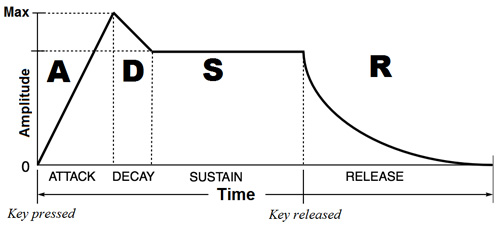
\includegraphics[width=\textwidth]{billeder/ADSR}
\end{center}

Som det ses af figuren har vi fire forskellige stadier: 
\begin{itemize}
\item Attack - Dette er i starten af signalet, hvor f.eks. en streng på en guitar bliver slået. Som vi kan se så stiger grafen kraftigt i Attack-stadiet. 
\item Decay - Her falder vores graf kraftigt, en smule, da vores streng på guitaren ikke kan holde den kraftige tone i så lang tid. Den skal falde ned til den stationære lyd, hvilket er det næste stadie.  
\item Sustain - Her holder vores graf et stationært niveau over noget tid. Dvs. at tonen, som vores guitar streng har givet, bliver holdt stabil over længere tid nu - Indtil tonen falder og dør ud (næste stadie). 
\item Release - Som vi kan se på vores graf dør vores signal ud her. Vores tone har altså holdt så længe den kan og dør nu ud efter det stabile-stadie. Så her falder og til sidst dør tonen ud. 
\end{itemize}

\section*{LFO}

Hvis vi så går videre til LFO: 

\begin{center}
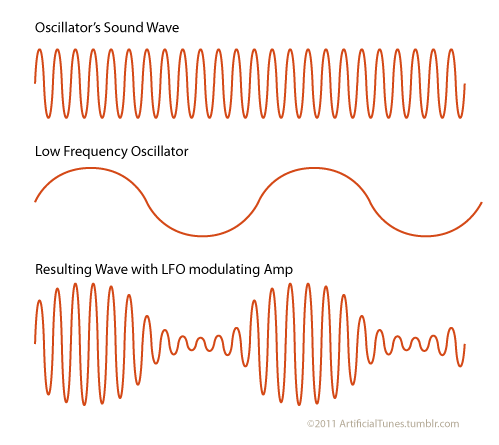
\includegraphics[width=\textwidth]{billeder/LFO}
\end{center}

Low-Frequency Oscillation er en anden måde at varierer amplituder på. 
Dette signal er for det meste under 20 Hz og bruges oftes til lydsignaler. Som navnet af denne metode siger, så bruger man altså kun dette når man har med lavere frekvenser at gøre. Frekvensen man benytter, når man skal have lavet sin sinusbølge, skal altid være lavere end tonen. 
Når man har fået lavet sin sinus kan vi beregne modeler sinus: 

$$S_mod (n) = (A_vo + 1)*s(n)$$
,hvor s(n) er vores sinus kurve. 

Herefter kan vi så beregne modulations graden, som betegnes, $f_L$.

Det skal så også siges at der er mange forskellige LFO-typer, det er ikke kun sinusser. Der er også firkants-, trekants-  og mange andre LFO-typer. 

\section*{Fourier transformation}
I DSB har vi nogle forskellige analyse værktøjer. Et af disse er Fourier transformation (DFT). Når vi benytter DFT regner vi med komplekse tal. 
Definitionen af DFT er betegnet: 
$$X(m)= \sum\limits_{n=0}^{N-1} x(n)*e^{-j*\frac{2*\pi}{N}*m*n}$$

,hvor m = frekvens nummerering. 



Det er altså sådan vi går fra tidsdomæne x(n), til frekvensdomæne X(m) - via Fourier transformation, DFT. 

Hvis vi så gerne vil tilbage igen, altså fra frekvensdomæne X(m), til tidsdonmæne x(n). Så laver vi Invers Fourier Transformation, IDFT. 
Definitionen af IDFT er betegnet: 
$$x(n)= \frac{1}{N} \sum\limits_{m=0}^{N-1} X(m)*e^{j*\frac{2*\pi}{N}*m*n}$$

Længden er = 1. 
Herefter er vi altså tilbage i tidsdomænet x(n).
\end{document}